\section{Studio di Finite Size Scaling}\label{Parte D}
A livello teorico è previsto un andamento della \emph{lunghezza di correlazione} in prossimità della temperatura critica del tipo:
\begin{equation}\label{eq: xivst}
\xi \propto \big| \dfrac{T - T_c}{T_c} \big|^{(-\nu)} = |t|^{(-\nu)}
\end{equation}
dove è stato introdotto il fattore $\nu$, detto \emph{esponenete critico}, che regola la divergenza ed è stimato essere  $\nu = 1$.

Ammettendo che sia la divergenza della lunghezza di correlazione a determinare il comportamento critico delle altre osservabili intorno a $T_c$ si potranno definire per tali quantità espressioni dello simili all' equazione (\ref{eq: xivst}) :

\begin{eqnarray}\label{eq: criticexpo}
 c & \propto & |t|^{-\alpha}  \propto \xi^{-\alpha / \nu}       \nonumber \\
 |M|  & \propto & \propto \xi^{-\beta / \nu}  \qquad (\textrm{\footnotesize{ solo per $T < T_c$}})\\
 \chi & \propto & |t|^{-\gamma}  \propto \xi^{-\gamma / \nu}
\end{eqnarray}

Il valore di questi esponenti critici non è stimabile in modo diretto ( attraverso un fit su punti campionati tramite delle simulazioni ad esempio) per via del vincolo della taglia finita che sta alla base di qualsiasi simulazione computazionale.
Non ci si aspetta che tale vincolo determini un generico cambiamento della dipendenza di $xi$ da $\beta$ ma che intervanga solamente causando un "cut-off" della divergenza della lunghezza di correlazione in prossimità alla temperatura critica.
Per un reticolo finito qualsiasi distanza non potrà essere maggiore della dimensione caratterisitica del sistema data dal lato del reticolo( la taglia $L$)\footnote{In realtà in presenza della condizione di bordo periodico la distanza massima che può essere sottesa tra due punti sarà $L/\sqrt{2}$}. Pertanto risulterà che:
\begin{equation}\label{eq: Xi_l}
\xi_L = \left\{ \begin{array}{rl}
 \xi_{\mbox{teo}}  &\mbox{ se $t \neq 0$} \\
  L &\mbox{ se $t \simeq 0$}
       \end{array} \right.
\end{equation}
\bigskip

Un criterio per stimare gli esponenti critici viene fornito dal metodo di \emph{Finite Size Scaling}.
Questa tecnica si basa sullo studio dell'andamento delle quantità osservabili in funzione della taglia $L$.
L'idea è la seguente: si consideri un osservabile critico, $\chi$ ad esempio, teoricamente la divergenza del valore d'aspettazione dipende dalla divergenza della lunghezza di correlazione secondo l'equazione \ref{eq: criticexpo} ma in un modello a taglia finita l'andamento di $\xi$ è limitato in accordo con l'equazione \ref{eq: Xi_l}. 
Unendo le due equazioni precedenti si ottiene il comportamento complessivo dell'osservabile $\chi$ per un sistema finito:
\begin{equation}\label{eq: Chi_finite}
\chi = \xi^{\gamma /\nu} \chi_0 (L/\xi)
\end{equation}
Nell'equazione è stata introdotta la funzione adimensionale $\chi_0:\mathbb{R} \rightarrow \mathbb{R}$ definita come:
\begin{equation}
\chi_0 (x) \propto \left\{ \begin{array}{rl}
		\mbox{cost}  &\mbox{ se $x \gg 1$} \\
  x^{-\gamma/\nu} &\mbox{ se $x \rightarrow 0$} \\
       \end{array} \right.
\end{equation}
la cui forma funzionale (incognita) rappresenta il modo esatto in cui il valore della suscettività viene smorzato per temperature vicino a $T_c$. 
La funzione è costruita in modo da non contere alcuna dipendenza implicita da $\xi$ che appare unicamente all'interno dell' argomento.

La dipendenza dalla lunghezza di correlazione può essere nascosta definendo una nuova funzione, detta \emph{di scaling},
\begin{equation}
\tilde{\chi}(x) = x^{-\gamma}\chi_0(x^{v}) \propto \left\{ \begin{array}{rl}
		x^{-\gamma}  &\mbox{ se $x \gg 1$} \\
  \mbox{cost} &\mbox{ se $x \rightarrow 0$} \\
       \end{array} \right.
\end{equation}
per cui risulta l'equazione:
\begin{equation}
\chi = L^{\gamma / \nu} \tilde{\chi}(L^{1/\nu} |t|)
\end{equation}
che descrive il modo in cui il valore di suscettività attorno alla temperatura critica varia in funzione di $L$.

\medskip
L'andamento preciso della funzione di scaling appena introdotta è incognito, ma per costruzione presenta due importanti proprietà:
\begin{itemize}
\item[-] La funzione di scaling è costante alla temperatura critica: 
		\begin{displaymath}
			\tilde{\chi}(x) \xrightarrow[x\rightarrow 0]{} x^{-\gamma}(x^\nu)^{\gamma/\nu} = \mbox{cost}
		\end{displaymath}
\item[-] La forma funzionale di $\tilde{\chi}$ non dipende da $L$. Pertanto il valore nell'origine ($T = T_c$) oltre ad essere costante è lo stesso per ogni sistema simulato a $L$ finito.
\end{itemize}

\medskip
Tutto questo può essere sfruttato per determinare gli esponenti critici: per prima cosa si campionano un buon numero di valori d'aspettazione degli osservabili critici ($\chi_L(t)$ , $c_L(t)$ e $M_L(t)$) intorno alla temperatura critica e per varie taglie $L$ finite. Per ciascuno di tali osservabili varrà la relazione:

\begin{displaymath}
	\tilde{O}(L^{1/ \nu} t ) = L^{\theta / \nu}O_L(t)
\end{displaymath}
(dove $\theta$ è l'esponente critico associato all'osservabile O).
Per ogni osservabile è possibile costruire un grafico ponendo come ascissa il valore $x = L^{1/ \nu} t $ e come ordinata
$y = L^{\theta / \nu}O_L(t)$. 
Questo grafico rappresenterà l'andamento della funzione di scaling incognita a condizione che gli esponenti $ \theta $ e $ \nu $ verranno scelti esattamente coincidenti al valore dell'esponente critico.
Confrontando i grafici a differente $L$ relativi allo stesso osservabile si può dare una stima degli esponenti critici come valori per cui tutti gli andamenti collassano alla medesima curva universale, caratteristica dell'osservabile preso in considerazione.
\medskip \newline
La stima degli esponenti critici è stata ottenuta ponendo i dati campionati in un foglio di calcolo\footnote{File: \emph{Finite Size Scaling.xls}} e osservando come cambia la forma dei grafici al variare degli esponenti $\theta$ e $\nu$. I valori per cui tutti i grafici collassano approssimativamente ad una sola curva costituisco una stima per gli esponenti critici.
Da questa analisi risultano i seguenti risultati:
\begin{center}
\begin{tabular}{|c|c|}
\hline
	$ \nu $ &= 1 $\pm$ 0,1 \\
\hline
	$ \alpha $ &= 0,1 $\pm$ 0,2 \\
\hline
	$ \beta $ &= 1,25 $\pm$ 0,02 \\
\hline
	$ \gamma $ &= 1,75 $\pm$ 0,01 \\
\hline
\end{tabular}
\end{center}
(l'errore è calcolato in modo qualitativo stimando l'intervallo di valori in cui l'accordo con la curva universale appare ottimale).
Nelle figure (\ref{fig: Chi_finitesize_1}), (\ref{fig: M_finitesize_1}) e (\ref{fig: c_finitesize_1}) è mostrato il confronto tra gli andamenti originali degli osservabili critici (in funzione di $t= (T-T_c) / T_c$) a varie taglie e la curva ottenuta tramite l'analisi di Finite Size che ha condotto alle stime precedenti.


\begin{figure}[htbp]
      \centering
      \caption[ParteD\_Ossvst.cpp $\;\rightarrow\;$ Chivst\_file.p ]{Studio di Finite Size Scaling dell'osservabile $\chi$.}\label{fig: Chi_finitesize_1}
	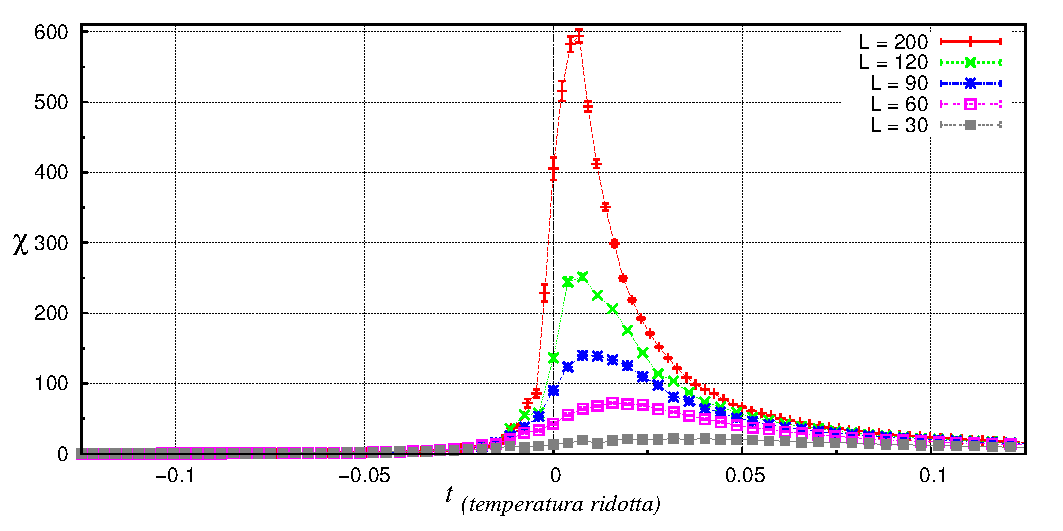
\includegraphics[width=1\textwidth]{Immagini/ParteD/Chivst}
	\bigskip
%	  \caption{}\label{fig: Chi_finitesize_2}
	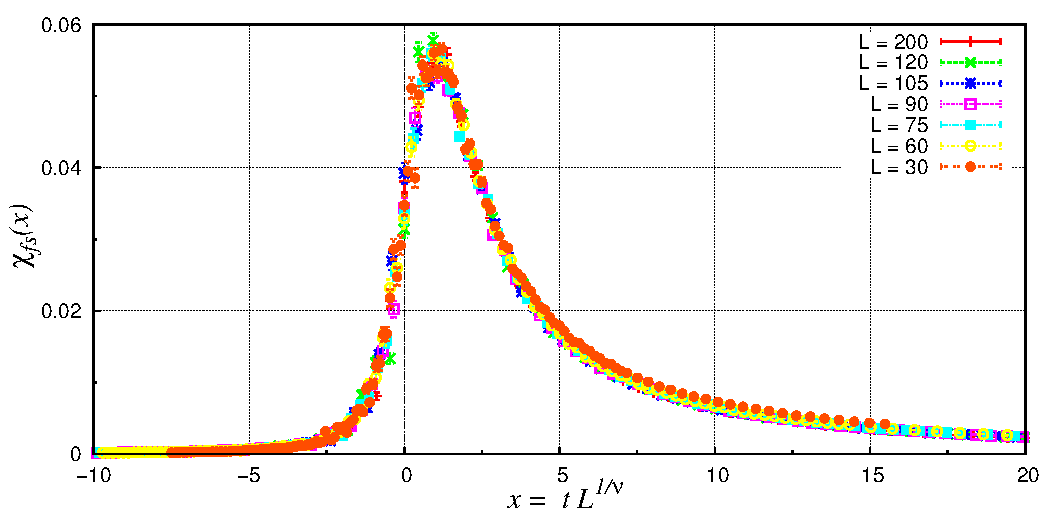
\includegraphics[width=1\textwidth]{Immagini/ParteD/Chivst_finite}
\end{figure}

\begin{figure}[htbp]
      \centering
      \caption[ParteD\_Ossvst.cpp $\;\rightarrow\;$ Mvst\_file.p ]{Studio di Finite Size Scaling dell'osservabile $M$.}\label{fig: M_finitesize_1}
	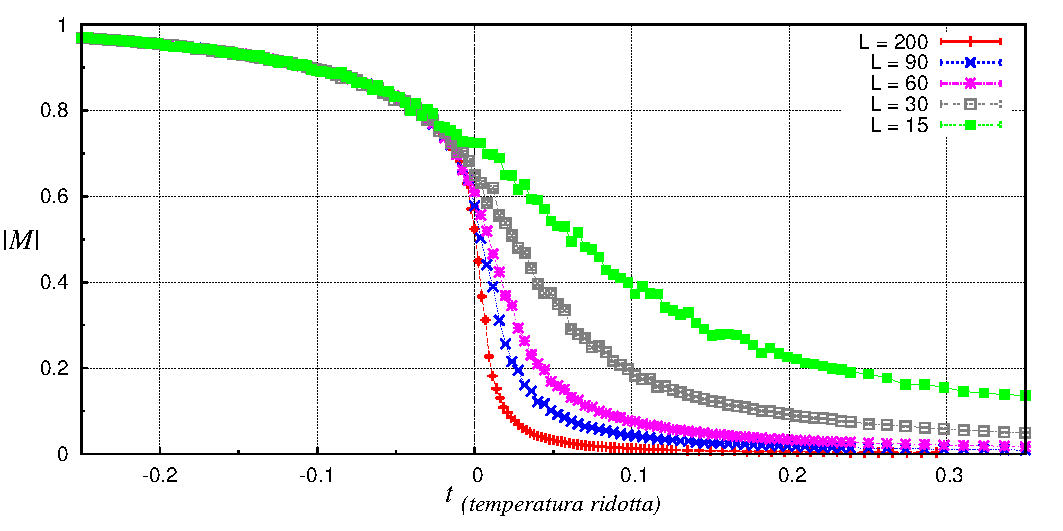
\includegraphics[width=1\textwidth]{Immagini/ParteD/Mvst}
	\bigskip
%	  \caption{}\label{fig: M_finitesize_2}
	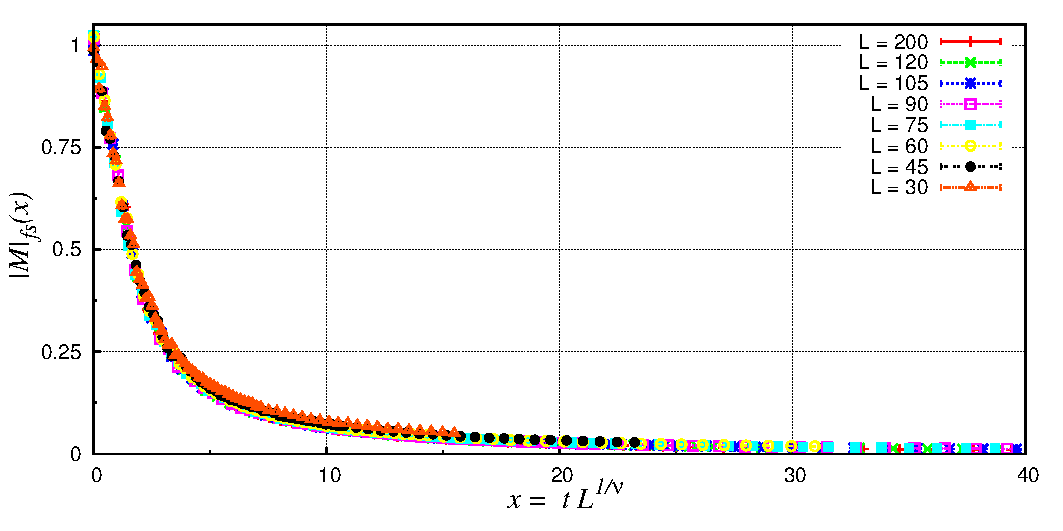
\includegraphics[width=1\textwidth]{Immagini/ParteD/Mvst_finite}
\end{figure}

\begin{figure}[htbp]
      \centering
      \caption[ParteD\_Ossvst.cpp $\;\rightarrow\;$ cvst\_file.p ]{Studio di Finite Size Scaling dell'osservabile $c$.}\label{fig: c_finitesize_1}
	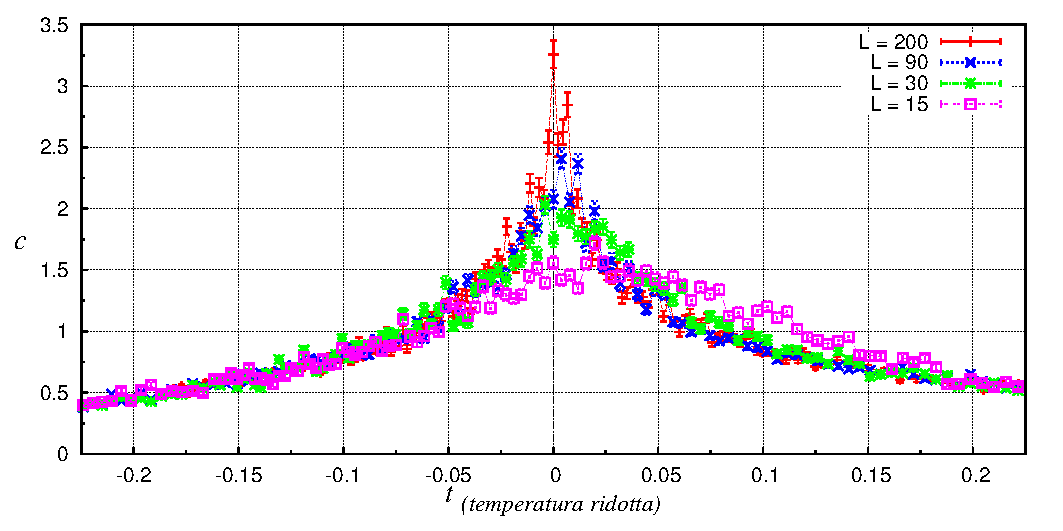
\includegraphics[width=1\textwidth]{Immagini/ParteD/cvst}
	\bigskip
%	  \caption{}\label{fig: c_finitesize_2}
	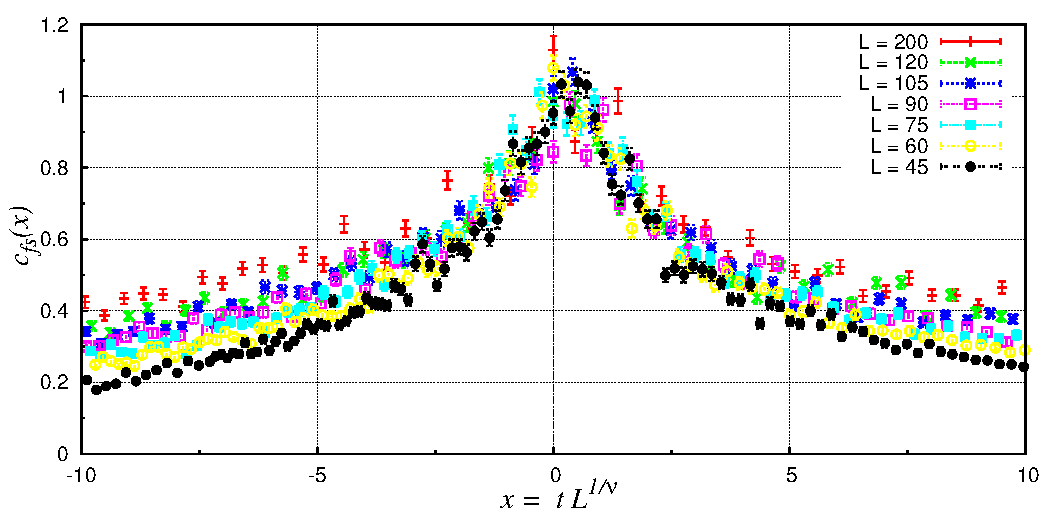
\includegraphics[width=1\textwidth]{Immagini/ParteD/cvst_finite}
\end{figure}

